\documentclass[aspectratio=169]{beamer}

% ===== Font and Encoding =====
\usepackage[utf8]{inputenc}
\usepackage[T1]{fontenc}
\usepackage{mathptmx} % Times New Roman + Math
\usepackage{helvet}   % Sans serif (for headers)
\usepackage{courier}  % Monospaced font
\renewcommand{\familydefault}{\rmdefault}

% ===== Packages =====
\usepackage{tikz}
\usetikzlibrary{shapes, arrows, positioning, shadows}
\usepackage{graphicx}
\usepackage{xcolor}
\usepackage{hyperref}
\usepackage{listings}
\usepackage{booktabs}
\usepackage{pifont}
\usepackage{colortbl}

% ===== Theme Customizations =====
\setbeamertemplate{navigation symbols}{}

\definecolor{tugreen}{RGB}{90,160,45}
\definecolor{lightgray}{RGB}{245,245,245}

% ===== Force all default Beamer text colors to black =====
\setbeamercolor{normal text}{fg=black,bg=white}
\setbeamercolor{structure}{fg=black}
\setbeamercolor{item}{fg=black}
\setbeamercolor{section in toc}{fg=black}
\setbeamercolor{subsection in toc}{fg=black}
\hypersetup{colorlinks=true, linkcolor=black, urlcolor=black}


% Footer
\setbeamertemplate{footline}{
    \leavevmode%
    \hbox{%
        \begin{beamercolorbox}[wd=\paperwidth, ht=3ex, dp=1.5ex, leftskip=1em, rightskip=1em, colsep*=1pt]{normal text}
            \vspace{-0.3ex}
            \hfill
            \insertframenumber
        \end{beamercolorbox}%
    }
}

% Header with logos + green bar
\setbeamertemplate{headline}{
    \begin{tikzpicture}[remember picture, overlay]
        % Left logo
        \node[anchor=north west, xshift=0.4cm, yshift=-0.3cm] at (current page.north west) {
            
\includegraphics[height=1cm]{abc/tudortmund.png}
        };
        % Right logo
        \node[anchor=north east, xshift=-0.4cm, yshift=-0.5cm] at (current page.north east) {
            
\includegraphics[height=0.8cm]{abc/cre.png}
        };
        % Green top line
        \fill[tugreen]
            ([xshift=0cm, yshift=-1.5cm] current page.north west)
            rectangle
            ([xshift=\paperwidth, yshift=-1.55cm] current page.north west);
    \end{tikzpicture}
    \vspace{1.5cm}
}

% Custom title page
\setbeamertemplate{title page}{
    \begin{tikzpicture}[remember picture, overlay]
        \node[anchor=north west, xshift=0.4cm, yshift=-0.3cm] at (current page.north west) {
            
\includegraphics[height=1cm]{abc/tudortmund.png}
        };
        \node[anchor=north east, xshift=-0.4cm, yshift=-0.5cm] at (current page.north east) {
            
\includegraphics[height=0.8cm]{abc/cre.png}
        };
        \fill[tugreen]
            ([xshift=0cm, yshift=-1.5cm] current page.north west)
            rectangle
            ([xshift=\paperwidth, yshift=-1.55cm] current page.north west);
    \end{tikzpicture}
    \vspace{4.5cm}
    \begin{center}
        {\usebeamerfont{title}\color{tugreen}\LARGE\textbf{\inserttitle}\par}
        \vspace{0.6cm}
        {\usebeamerfont{subtitle}\large\color{black!80}\insertsubtitle\par}
        \vspace{1cm}
        {\large\textit{\insertauthor}}\par
        {\small\insertdate}
    \end{center}
}

% ===== Listings style =====
\lstset{
    basicstyle=\ttfamily\small,
    keywordstyle=\color{tugreen}\bfseries,
    commentstyle=\color{gray}\itshape,
    stringstyle=\color{orange},
    numbers=left,
    numberstyle=\tiny\color{gray},
    numbersep=8pt,
    frame=single,
    rulecolor=\color{gray!50},
    breaklines=true,
    showstringspaces=false,
    tabsize=2,
    backgroundcolor=\color{gray!10}
}

% ===== TikZ Styles =====
\tikzstyle{process}  = [rectangle, minimum width=2.5cm, minimum height=1cm, text centered, draw=black, fill=white]
\tikzstyle{guistep}  = [rectangle, rounded corners, minimum width=3.2cm, minimum height=0.9cm,
                        text centered, draw=tugreen, fill=tugreen!15, font=\small\bfseries]
\tikzstyle{arrow}    = [thick,->,>=stealth]

% ===== Title Information =====
\title{PFEM Benchmark Catalogue}
\subtitle{From Deterministic Sweeps to Probabilistic Analysis}
\author{Naty Manque \& Naeem Zainuddin}
\date{June 2026}

% ===== Document Start =====
\begin{document}

% ---------------------------------------------------------
% 1. Title
% ---------------------------------------------------------
\begin{frame}[plain]
    \titlepage
\end{frame}

% ---------------------------------------------------------
% 1b. Progress Roadmap
% ---------------------------------------------------------
\begin{frame}{Where We Are}
    \begin{columns}[t]
        \begin{column}{0.52\textwidth}
            \textbf{Done}
            \begin{itemize}
                \setlength\itemsep{0.35em}
                \item[\textcolor{tugreen}{\ding{51}}] \textbf{Foundation:} all 87 PFEM cases build, run and verified on Linux
                \item[\textcolor{tugreen}{\ding{51}}] \textbf{Deterministic sweeps} + 3D post-processing \\(demo today: p6.12 slope)
                \item[\textcolor{tugreen}{\ding{51}}] \textbf{Phase~1:} universal Quantity-of-Interest extraction + Monte~Carlo
                \item[\textcolor{tugreen}{\ding{51}}] \textbf{Phase~2:} Latin Hypercube, correlated inputs, sensitivity tornado
            \end{itemize}
        \end{column}
        \begin{column}{0.46\textwidth}
            \textbf{Next}
            \begin{itemize}
                \setlength\itemsep{0.35em}
                \item Phase~3: pluggable runner for non-PFEM codes
                \item Phase~4: mesh-refinement convergence studies
                \item Regression testing vs reference outputs
            \end{itemize}
            \vspace{0.4cm}
            \textbf{Handover:} complete documentation set and a 3-minute reproducible test, all on GitHub (final slides).
        \end{column}
    \end{columns}

    \vspace{0.3cm}
    \centering
    {\small The story: we went from \emph{one number per run} to \emph{full probabilistic and sensitivity analysis} across every case.}
\end{frame}

% ---------------------------------------------------------
% 2. What We Built (one concise slide)
% ---------------------------------------------------------
\begin{frame}{How It Works --- One Pipeline, Five Stages}
    \centering
    \vspace{0.2cm}
    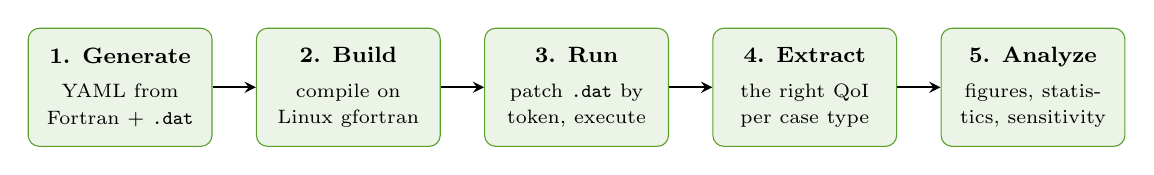
\begin{tikzpicture}[font=\footnotesize]
        \tikzstyle{stg}=[rectangle, rounded corners, draw=tugreen, fill=tugreen!12,
                         minimum width=2.25cm, minimum height=1.5cm, text centered,
                         text width=2.1cm, font=\footnotesize]
        \node (g) [stg] {\textbf{1. Generate}\\[3pt]{\scriptsize YAML from Fortran + \texttt{.dat}}};
        \node (b) [stg, right=0.55cm of g] {\textbf{2. Build}\\[3pt]{\scriptsize compile on Linux gfortran}};
        \node (r) [stg, right=0.55cm of b] {\textbf{3. Run}\\[3pt]{\scriptsize patch \texttt{.dat} by token, execute}};
        \node (e) [stg, right=0.55cm of r] {\textbf{4. Extract}\\[3pt]{\scriptsize the right QoI per case type}};
        \node (a) [stg, right=0.55cm of e] {\textbf{5. Analyze}\\[3pt]{\scriptsize figures, statistics, sensitivity}};
        \draw[arrow] (g)--(b);
        \draw[arrow] (b)--(r);
        \draw[arrow] (r)--(e);
        \draw[arrow] (e)--(a);
    \end{tikzpicture}

    \vspace{0.5cm}
    \begin{columns}[t]
        \begin{column}{0.48\textwidth}
            \textbf{Key idea}
            \begin{itemize}
                \setlength\itemsep{0.25em}
                \item YAML is the bridge: parameters patched by \textbf{token index}
                \item The Fortran \textbf{source is never edited}
                \item One driver runs all \textbf{87} cases
            \end{itemize}
        \end{column}
        \begin{column}{0.48\textwidth}
            \textbf{Same core, four modes}
            \begin{itemize}
                \setlength\itemsep{0.25em}
                \item Deterministic sweep
                \item Monte Carlo \,/\, Latin Hypercube
                \item Correlated sampling
                \item One-at-a-time sensitivity
            \end{itemize}
        \end{column}
    \end{columns}

    \vspace{0.3cm}
    \centering
    {\small \textbf{Demo today:} 3D slope stability (p6.12) --- Mohr-Coulomb with strength reduction}
\end{frame}

% =========================================================
% Case Study: p6.12
% =========================================================

% ---------------------------------------------------------
% 3. p6.12 Problem Setup
% ---------------------------------------------------------
\begin{frame}[shrink=5]{p6.12 --- 3D Slope Stability (Mohr-Coulomb)}
    \begin{columns}[t]
        \begin{column}{0.54\textwidth}
            \textbf{Physical Problem}
            \begin{itemize}
                \setlength\itemsep{0.3em}
                \item 3D embankment slope, elastic-perfectly plastic
                \item Mohr-Coulomb failure criterion with 5 material zones
                \item Hex8 mesh, 20-point Gaussian integration
            \end{itemize}

            \vspace{0.4cm}
            \textbf{Strength Reduction Factor (SRF)}

            Shear strength is scaled down uniformly at each step:
            \[
                \hat{c} = \frac{c}{\text{SRF}}, \qquad
                \tan\hat{\phi} = \frac{\tan\phi}{\text{SRF}}
            \]
            Failure = last SRF at which Newton-Raphson converges.

            \vspace{0.2cm}
            \textbf{Sweep:} 4 scenarios varying $c$ ($\phi=20^\circ$ fixed).
        \end{column}
        \begin{column}{0.42\textwidth}
            \textbf{Default Parameters}
            \begin{center}
            \small
            \begin{tabular}{ll}
                \toprule
                Parameter & Value \\
                \midrule
                Cohesion $c$       & 60 kPa \\
                Friction $\phi$    & 20$^\circ$ \\
                Dilation $\psi$    & 0$^\circ$ \\
                Young's $E$        & $10^5$ Pa \\
                Poisson $\nu$      & 0.3 \\
                SRF range          & 1.0 -- 1.60 \\
                Iteration limit    & 1000 \\
                \bottomrule
            \end{tabular}
            \end{center}
        \end{column}
    \end{columns}
\end{frame}

% ---------------------------------------------------------
% 4. Material Zones
% ---------------------------------------------------------
\begin{frame}{p6.12 --- Material Zones}
    \begin{columns}[c]
        \begin{column}{0.58\textwidth}
            \includegraphics[width=\textwidth]{../runs/chap06/p612/p612_sweep_20260325_231409_ensi_zones_single.png}
        \end{column}
        \begin{column}{0.40\textwidth}
            \textbf{5 horizontal soil layers}
            \begin{itemize}
                \setlength\itemsep{0.4em}
                \item Each zone has its own cohesion $c$ and friction angle $\phi$
                \item Geometry is \textbf{identical} across all sweep scenarios
                \item Only the base cohesion value changes; zone proportions are preserved
                \item Slope face visible on the right side
            \end{itemize}
        \end{column}
    \end{columns}
\end{frame}

% ---------------------------------------------------------
% 5. SRF Curves
% ---------------------------------------------------------
\begin{frame}[shrink=5]{p6.12 --- SRF Curves (Sweep Output)}
    \begin{columns}[c]
        \begin{column}{0.58\textwidth}
            \includegraphics[width=\textwidth]{../runs/chap06/p612/p612_sweep_20260325_231409_res_overlay.pdf}
        \end{column}
        \begin{column}{0.40\textwidth}
            \textbf{What this shows}
            \begin{itemize}
                \setlength\itemsep{0.35em}
                \item X-axis: Strength Reduction Factor applied to $c$ and $\phi$
                \item Y-axis: maximum displacement $\delta_\text{max}$
                \item \textcolor{blue}{$c{=}50$\,kPa}: slope fails at SRF${\approx}1.4$ --- displacement diverges
                \item \textcolor{red}{$c{=}60$\,kPa} (book): FS${\approx}1.6$
                \item \textcolor[rgb]{0.17,0.63,0.17}{$c{=}75$}, \textcolor{orange}{$c{=}90$}: stable --- no divergence
            \end{itemize}
            \vspace{0.2cm}
            {\small \textbf{Key:} diverging $\delta_\text{max}$ signals slope failure.}
        \end{column}
    \end{columns}
\end{frame}

% (3D deformed-mesh overview and c=50 / c=60 zoom slides moved to the appendix
%  to keep the main deck concise.)

% ---------------------------------------------------------
% 9. Verification vs. Book
% ---------------------------------------------------------
\begin{frame}{p6.12 --- Verification vs.\ Book (Figs.~6.54--6.55)}
    \begin{columns}[t]
        \begin{column}{0.50\textwidth}
            \textbf{SRF vs.\ Max Displacement} ($c{=}60$, $\phi{=}20^\circ$)
            \begin{center}
            \small
            \begin{tabular}{rcc}
                \toprule
                SRF & $\delta_\text{max}$ & Iterations \\
                \midrule
                1.00 & $0.02266$ & 16 \\
                1.40 & $0.03123$ & 77 \\
                1.50 & $0.03930$ & 208 \\
                1.55 & $0.04971$ & 380 \\
                1.58 & $0.06363$ & 703 \\
                1.60 & $0.09308$ & 1000 \\
                \bottomrule
            \end{tabular}
            \end{center}
            \vspace{0.15cm}
            Failure at SRF $\approx 1.58$--$1.60$
        \end{column}
        \begin{column}{0.46\textwidth}
            \textbf{Verification}
            \begin{itemize}
                \setlength\itemsep{0.5em}
                \item[\textcolor{tugreen}{\ding{51}}] SRF--displacement curve matches book Fig.~6.54
                \item[\textcolor{tugreen}{\ding{51}}] Failure SRF $\approx 1.58$--$1.60$ agrees with reference
                \item[\textcolor{tugreen}{\ding{51}}] 3D slip surface visible in deformed mesh (Fig.~6.55)
                \item[\textcolor{tugreen}{\ding{51}}] Iteration count growth consistent with limit-state analysis
            \end{itemize}
        \end{column}
    \end{columns}
\end{frame}

% =========================================================
% NEW: Phase 1 & 2 -- Probabilistic and Sensitivity Analysis
% =========================================================

% ---- Phase 1 concept: universal QoI + Monte Carlo ----
\begin{frame}{Phase 1 --- From One Answer to a Distribution}
    \begin{columns}[t]
        \begin{column}{0.52\textwidth}
            \textbf{The problem}
            \begin{itemize}
                \setlength\itemsep{0.3em}
                \item A deterministic run gives \emph{one} number for \emph{one} set of inputs
                \item Real material properties are uncertain (scatter, test variability)
                \item The old extractor only understood slope-stability output
            \end{itemize}
            \vspace{0.25cm}
            \textbf{What was added}
            \begin{itemize}
                \setlength\itemsep{0.3em}
                \item[\textcolor{tugreen}{\ding{51}}] A \textbf{universal QoI extractor}: pulls the right physical answer for \textbf{all 87} cases (8 case types)
                \item[\textcolor{tugreen}{\ding{51}}] \textbf{Monte Carlo}: sample inputs from distributions, get a distribution of answers
            \end{itemize}
        \end{column}
        \begin{column}{0.46\textwidth}
            \textbf{Case type $\to$ Quantity of Interest}
            \begin{center}
            \scriptsize
            \begin{tabular}{ll}
                \toprule
                Case type & QoI \\
                \midrule
                Slope stability     & Factor of Safety \\
                Plasticity          & Limit load \\
                Elastic             & Max displacement \\
                Seepage             & Max head \\
                Consolidation       & Degree of consol. \\
                Eigenvalue          & $\omega^2$ (and $f_1$) \\
                Dynamics            & Peak displacement \\
                Thermal             & Max temperature \\
                \bottomrule
            \end{tabular}
            \end{center}
            {\scriptsize \textbf{87 / 87} cases return a meaningful QoI from their default run.}
        \end{column}
    \end{columns}
\end{frame}

% ---- Phase 1 result: FS distribution + reliability ----
\begin{frame}{Phase 1 --- Result: Slope Reliability (p6.12)}
    \begin{columns}[c]
        \begin{column}{0.58\textwidth}
            \includegraphics[width=\textwidth]{../runs/chap06/p612/p612_stochastic_20260507_150058_fs_hist.png}
        \end{column}
        \begin{column}{0.40\textwidth}
            \textbf{Cohesion sampled as lognormal}
            \begin{itemize}
                \setlength\itemsep{0.35em}
                \item Each Monte Carlo sample runs the full 3D Fortran solver
                \item Output: a \textbf{distribution} of Factor of Safety, not a single value
                \item Gives \textbf{probability of failure} $P(\text{FS}<1)$ and reliability index $\beta$
            \end{itemize}
            \vspace{0.2cm}
            {\small This is the language a geotechnical reviewer actually wants: not "FS = 1.58" but "probability of failure = X\%".}
        \end{column}
    \end{columns}
\end{frame}

% ---- Phase 2.1: LHS variance reduction + scatter ----
\begin{frame}{Phase 2 --- Latin Hypercube: Same Cost, Better Coverage}
    \begin{columns}[c]
        \begin{column}{0.50\textwidth}
            \includegraphics[width=\textwidth]{../runs/chap06/p612/p612_stochastic_20260507_150058_fs_scatter_cohesion_c.png}
        \end{column}
        \begin{column}{0.48\textwidth}
            \textbf{Variance reduction vs plain Monte Carlo}
            \begin{center}
            \small
            \begin{tabular}{rcc}
                \toprule
                Samples & LHS std & IID std \\
                \midrule
                25  & 0.75 & 4.92 \quad(\textbf{6.5$\times$}) \\
                50  & 0.54 & 3.42 \\
                100 & 0.20 & 2.33 \\
                200 & 0.11 & 1.58 \quad(\textbf{14$\times$}) \\
                \bottomrule
            \end{tabular}
            \end{center}
            \vspace{0.2cm}
            \begin{itemize}
                \setlength\itemsep{0.3em}
                \item Same number of expensive Fortran runs
                \item 6--14$\times$ tighter estimate of the mean
                \item Scatter (left) shows FS rising smoothly with cohesion --- physically correct
            \end{itemize}
        \end{column}
    \end{columns}
\end{frame}

% ---- Phase 2.2: correlated inputs ----
\begin{frame}{Phase 2 --- Correlated Inputs (Iman--Conover)}
    \begin{columns}[t]
        \begin{column}{0.50\textwidth}
            \textbf{Why}
            \begin{itemize}
                \setlength\itemsep{0.3em}
                \item In real soils, cohesion $c$ and friction $\phi$ are correlated (typically negatively)
                \item Sampling them independently is unphysical
                \item Iman--Conover induces a \textbf{target correlation} while keeping each input's distribution exact
            \end{itemize}
        \end{column}
        \begin{column}{0.48\textwidth}
            \textbf{Reproduced target correlations ($n{=}500$)}
            \begin{center}
            \small
            \begin{tabular}{cc}
                \toprule
                Target $\rho$ & Observed $\rho$ \\
                \midrule
                $-0.70$ & $-0.654$ \\
                $-0.30$ & $-0.275$ \\
                $+0.00$ & $-0.002$ \\
                $+0.50$ & $+0.494$ \\
                \bottomrule
            \end{tabular}
            \end{center}
            \vspace{0.2cm}
            {\small Targets in $[-0.7,+0.5]$ reproduced within 5\%, marginals preserved exactly.}
        \end{column}
    \end{columns}
\end{frame}

% ---- Phase 2.3: sensitivity tornado ----
\begin{frame}{Phase 2 --- Sensitivity: Which Input Matters?}
    \begin{columns}[c]
        \begin{column}{0.58\textwidth}
            \includegraphics[width=\textwidth]{../runs/chap06/p612/p612_tornado_3param_20260515_124907.png}
        \end{column}
        \begin{column}{0.40\textwidth}
            \textbf{One-at-a-time tornado (p6.12)}
            \begin{itemize}
                \setlength\itemsep{0.35em}
                \item Each input varied $\pm 1\sigma$; bar length = effect on FS
                \item \textbf{Cohesion} dominates (spread 0.58)
                \item \textbf{$E$ and $\nu$} have \emph{zero} effect on FS
            \end{itemize}
            \vspace{0.2cm}
            {\small Exactly the textbook expectation: in strength-reduction analysis only strength parameters move the safety factor; stiffness only affects displacements. The tool \textbf{recovers the physics}.}
        \end{column}
    \end{columns}
\end{frame}

% ---- Validation summary ----
\begin{frame}{Why We Trust It --- Validation}
    \begin{center}
    \small
    \begin{tabular}{lccc}
        \toprule
        Case & Computed & Reference & Match \\
        \midrule
        p6.12 slope FS ($c{=}60$, $\phi{=}0$) & 1.58 & Book Fig.~6.54 & \textcolor{tugreen}{\ding{51}} \\
        p6.1 limit load ($\sigma_y{=}100$)    & 515 & Prandtl $(2{+}\pi)\sigma_y = 514$ & \textcolor{tugreen}{\ding{51}}\ 0.2\% \\
        p10.1 beam $\omega^2$                 & 0.00382 & Analytic cantilever 0.00402 & \textcolor{tugreen}{\ding{51}} \\
        LHS variance reduction                & 6.5--14$\times$ & McKay et al.\ (1979) & \textcolor{tugreen}{\ding{51}} \\
        Correlation reproduction             & within 5\% & Iman--Conover (1982) & \textcolor{tugreen}{\ding{51}} \\
        \bottomrule
    \end{tabular}
    \end{center}
    \vspace{0.4cm}
    \begin{itemize}
        \setlength\itemsep{0.3em}
        \item Results match the \textbf{textbook} and \textbf{analytical} solutions, not just "it runs"
        \item A single 3-minute script (\texttt{test\_phase2\_multi\_case.m}) reproduces this evidence on demand
    \end{itemize}
\end{frame}

% ---- Handover ----
\begin{frame}{Handover --- Anyone Can Pick This Up}
    \begin{columns}[t]
        \begin{column}{0.52\textwidth}
            \textbf{Everything is documented and on GitHub}
            \begin{itemize}
                \setlength\itemsep{0.3em}
                \item \texttt{ARCHITECTURE.md} --- end-to-end flow, how every file connects, the call graph, every problem solved
                \item \texttt{HANDOVER.md} --- fresh-machine setup, status, gotchas
                \item \texttt{GUIDE.md} / \texttt{matlab/README.md} --- usage and function reference
                \item \texttt{PROGRESS.md} --- this validation evidence in full
            \end{itemize}
        \end{column}
        \begin{column}{0.46\textwidth}
            \textbf{Reproducible from a cold start}
            \begin{itemize}
                \setlength\itemsep{0.3em}
                \item A literal "\textbf{zero to first result}" runbook: clone $\to$ build $\to$ run $\to$ figure
                \item 3-minute test script reproduces all validation
                \item Documented patches make the textbook Fortran compile on Linux
            \end{itemize}
            \vspace{0.3cm}
            {\small The only thing not in the repo is the licensed PFEM source --- but the exact patches to rebuild it are.}
        \end{column}
    \end{columns}
\end{frame}

% ---------------------------------------------------------
% 10. Conclusions
% ---------------------------------------------------------
\begin{frame}{Conclusions \& Next Steps}
    \begin{columns}[t]
        \begin{column}{0.48\textwidth}
            \textbf{What was achieved}
            \begin{itemize}
                \setlength\itemsep{0.4em}
                \item[\textcolor{tugreen}{\ding{51}}] 87 PFEM benchmarks verified on Linux (token-based YAML, zero source changes)
                \item[\textcolor{tugreen}{\ding{51}}] Universal QoI extraction across all 8 case types
                \item[\textcolor{tugreen}{\ding{51}}] Monte Carlo + Latin Hypercube + correlated inputs
                \item[\textcolor{tugreen}{\ding{51}}] One-at-a-time sensitivity (tornado) recovering the physics
                \item[\textcolor{tugreen}{\ding{51}}] Validated vs textbook and analytical solutions
                \item[\textcolor{tugreen}{\ding{51}}] Full handover documentation on GitHub
            \end{itemize}
        \end{column}
        \begin{column}{0.48\textwidth}
            \textbf{Next steps}
            \begin{itemize}
                \setlength\itemsep{0.45em}
                \item Phase 3: pluggable runner for non-PFEM codes
                \item Phase 4: mesh-resolution convergence sweeps ($nxe$, $nye$)
                \item Automated regression testing against reference outputs
                \item User-selectable probe node for boundary-bound QoIs
            \end{itemize}
        \end{column}
    \end{columns}
\end{frame}

% ---------------------------------------------------------
% 11. Thank You
% ---------------------------------------------------------
\begin{frame}
    \centering
    \vspace{2.5cm}
    {\Huge Thank You!}\\[1cm]
    {\large Questions?}
\end{frame}

% =========================================================
% APPENDIX --- Backup Slides
% =========================================================
\appendix

\begin{frame}
    \centering
    \vspace{3cm}
    {\Large\textbf{Backup Slides}}
\end{frame}

% ---- Pipeline & GUI (moved from main) ----

\begin{frame}[shrink=8]{Pipeline Architecture}
    \centering
    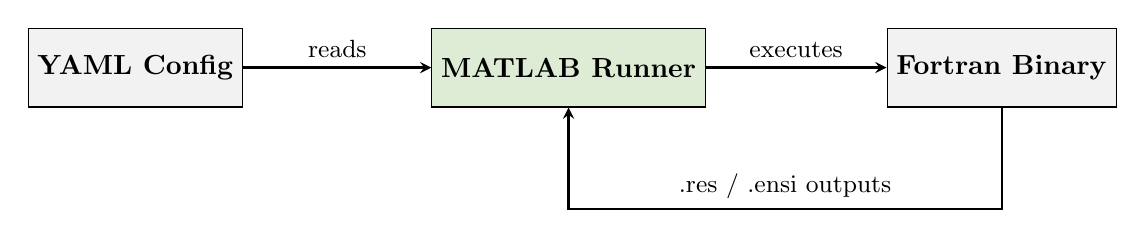
\begin{tikzpicture}[node distance=2.5cm, auto]
        \node (yaml)    [process, fill=gray!10]      {\textbf{YAML Config}};
        \node (matlab)  [process, right of=yaml,   xshift=3cm, fill=tugreen!20] {\textbf{MATLAB Runner}};
        \node (fortran) [process, right of=matlab, xshift=3cm, fill=gray!10]   {\textbf{Fortran Binary}};

        \draw [arrow] (yaml)    -- node[above] {\small reads} (matlab);
        \draw [arrow] (matlab)  -- node[above] {\small executes} (fortran);
        \draw [arrow] (fortran) -- ++(0,-1.8) -| node[pos=0.25, above] {\small .res / .ensi outputs} (matlab);
    \end{tikzpicture}

    \vspace{0.5cm}
    \raggedright
    \textbf{YAML acts as the bridge between rigid Fortran and flexible MATLAB.}

    \vspace{0.3cm}
    \begin{columns}[t]
        \begin{column}{0.48\textwidth}
            \textbf{Per-run steps}
            \begin{enumerate}
                \setlength\itemsep{0.3em}
                \item Locate binary + template \texttt{.dat}
                \item Copy to an isolated sandbox folder
                \item Inject override values as positional tokens
                \item Execute; parse output files
            \end{enumerate}
        \end{column}
        \begin{column}{0.48\textwidth}
            \textbf{Example tunable tokens}
            \begin{itemize}
                \setlength\itemsep{0.3em}
                \item \texttt{youngs\_modulus\_E} $\to$ replaces value in \texttt{.dat}
                \item \texttt{cohesion\_c}, \texttt{friction\_phi} $\to$ MC sweep
                \item One YAML, many scenarios --- no manual editing
            \end{itemize}
        \end{column}
    \end{columns}
\end{frame}

\begin{frame}{Sweep GUI --- \texttt{pfem\_sweep\_gui}}
    \begin{columns}[c]
        \begin{column}{0.54\textwidth}
            A single MATLAB interface for all 87 benchmark cases:
            \begin{itemize}
                \setlength\itemsep{0.4em}
                \item Browse cases by chapter; inspect tunables with suggested ranges
                \item Define sweeps on a \textbf{log or linear} grid
                \item Execute variants in isolated sandboxes
                \item Auto-generate summary figures (mesh, displacement, SRF, 3D EnSight)
            \end{itemize}
        \end{column}
        \begin{column}{0.42\textwidth}
            \centering
            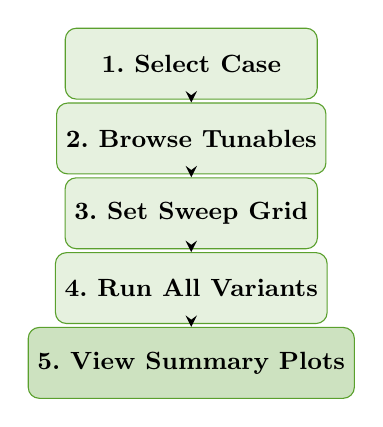
\begin{tikzpicture}[node distance=0.95cm]
                \node (a) [guistep] {1.\ Select Case};
                \node (b) [guistep, below of=a] {2.\ Browse Tunables};
                \node (c) [guistep, below of=b] {3.\ Set Sweep Grid};
                \node (d) [guistep, below of=c] {4.\ Run All Variants};
                \node (e) [guistep, below of=d, fill=tugreen!30] {5.\ View Summary Plots};
                \draw[arrow] (a)--(b); \draw[arrow] (b)--(c);
                \draw[arrow] (c)--(d); \draw[arrow] (d)--(e);
            \end{tikzpicture}
        \end{column}
    \end{columns}
\end{frame}

\begin{frame}[plain]
    \begin{tikzpicture}[remember picture, overlay]
        \node[anchor=center] at (current page.center) {
            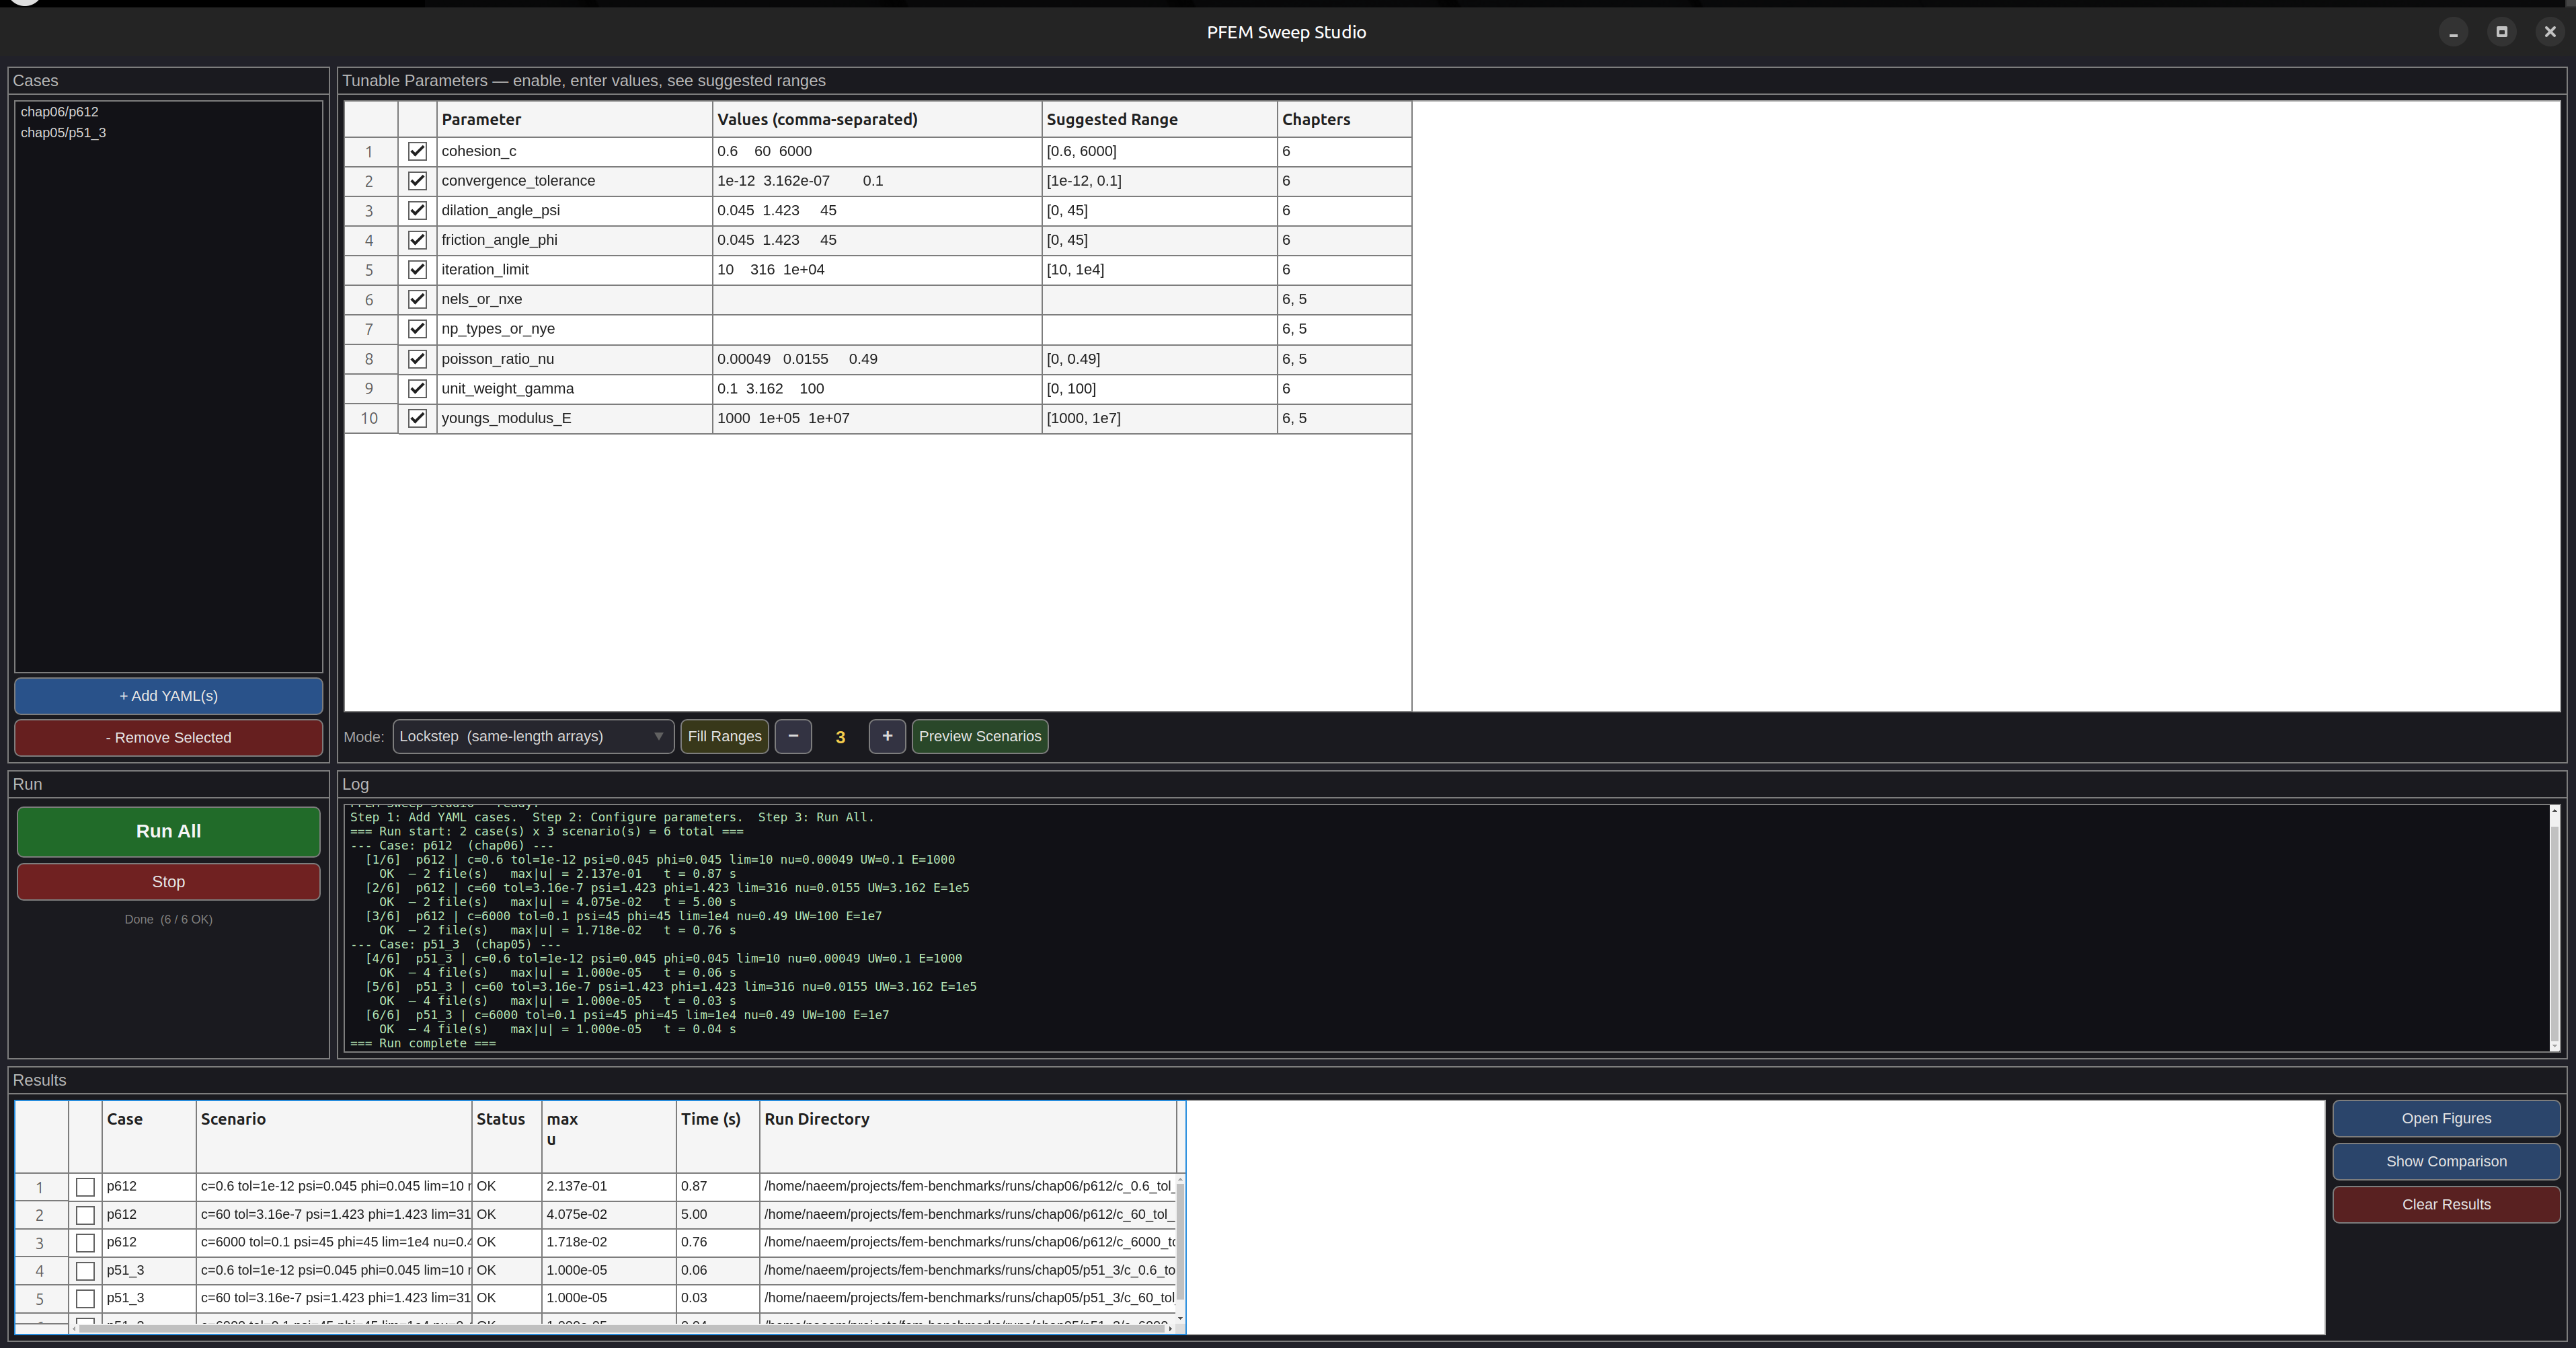
\includegraphics[width=\paperwidth, height=\paperheight, keepaspectratio]{abc/gui.png}
        };
    \end{tikzpicture}
\end{frame}

% ---- Background ----

\begin{frame}[shrink=5]{Problem Statement}
    Developing benchmark Fortran codes (PFEM, 5th ed.) by automating YAML metadata generation to tokenise \texttt{.dat} inputs.

    \vspace{0.4cm}
    \begin{columns}[t]
        \begin{column}{0.48\textwidth}
            \textbf{Key Challenges}
            \begin{itemize}
                \setlength\itemsep{0.3em}
                \item \textbf{Legacy Input:} Unstructured \texttt{.dat} files.
                \item \textbf{Opaque Parsing:} The \texttt{read10} subroutine hides logic.
                \item \textbf{Constraint:} Source code must remain untouched.
            \end{itemize}
        \end{column}
        \begin{column}{0.48\textwidth}
            \textbf{Objectives}
            \begin{itemize}
                \setlength\itemsep{0.3em}
                \item \textbf{Reproducibility:} Run any case reliably.
                \item \textbf{Interoperability:} Drive execution via MATLAB.
                \item \textbf{Searchability:} Consistent YAML metadata.
            \end{itemize}
        \end{column}
    \end{columns}
\end{frame}

\begin{frame}{Path to Completion}
    To transition from prototype to a \textbf{research-ready benchmark repository}:

    \vspace{0.3cm}
    \begin{enumerate}
        \setlength\itemsep{0.5em}
        \item \textbf{Standardise YAML Schema (All Chapters)}
        \begin{itemize}
            \item Uniform metadata keys and consistent tunable definitions.
        \end{itemize}
        \item \textbf{Define Scope of Tunables}
        \begin{itemize}
            \item \textbf{Phase 1:} Material props ($E, \nu, k$), loads.
            \item \textbf{Phase 2:} Mesh resolution ($nxe$, $nye$).
        \end{itemize}
        \item \textbf{Implement Validation Layer}
        \begin{itemize}
            \item Health checks and regression testing against reference outputs.
        \end{itemize}
    \end{enumerate}
\end{frame}

% ---- p5.1 Case Study ----

\begin{frame}[fragile,shrink=5]{p5.1 --- Problem Setup (Linear Elasticity 2D)}
    \begin{columns}[t]
        \begin{column}{0.52\textwidth}
            \textbf{Physical Problem}
            \begin{itemize}
                \setlength\itemsep{0.3em}
                \item Plane-stress elastic solid under point loads
                \item Mesh: $3 \times 2$ bilinear quadrilateral elements (12 nodes, 6 elements)
                \item Fixed bottom edge; two point loads applied at top
            \end{itemize}

            \vspace{0.2cm}
            \textbf{Tunable Parameters}
            \begin{center}
            \small
            \begin{tabular}{lcc}
                \toprule
                Parameter & Symbol & Range \\
                \midrule
                Young's modulus & $E$ & $10^4$--$10^8$ \\
                Poisson's ratio & $\nu$ & $5{\times}10^{-4}$--$0.49$ \\
                \bottomrule
            \end{tabular}
            \end{center}
            \vspace{0.1cm}
            {\small Sweep: 4 combinations on a log grid.}
        \end{column}
        \begin{column}{0.44\textwidth}
            \textbf{YAML snippet}
            \begin{lstlisting}[language={}, basicstyle=\ttfamily\tiny, numbers=none, frame=single]
id: pfem5_ch05_p51_p51_3
title: PFEM p51 -- case p51_3
purpose: Linear Elasticity 2D

tunable_parameters:
- name: youngs_modulus_E
  current_value: '1.0e6'
  suggested_range: [1e4, 1e9]
- name: poisson_ratio_nu
  current_value: '0.3'
  suggested_range: [0.0, 0.49]
            \end{lstlisting}
        \end{column}
    \end{columns}
\end{frame}

\begin{frame}{p5.1 --- Load--Displacement Overlay}
    \begin{columns}[c]
        \begin{column}{0.58\textwidth}
            \includegraphics[width=\textwidth]{../runs/chap05/p51_3/p51_3_sweep_20260325_220808_res_overlay.pdf}
        \end{column}
        \begin{column}{0.40\textwidth}
            \textbf{What this shows}
            \begin{itemize}
                \setlength\itemsep{0.4em}
                \item 4 scenarios: $E$ and $\nu$ varied on a log grid
                \item \textcolor{orange}{$\nu{=}0.49$}: near-incompressible, strong Poisson effect
                \item Low $\nu$ scenarios cluster together --- stiffness dominates
            \end{itemize}
        \end{column}
    \end{columns}
\end{frame}

\begin{frame}{p5.1 --- Deformed Shapes (All Scenarios)}
    \vspace{-0.2cm}
    \begin{center}
        \includegraphics[width=0.96\textwidth, height=0.72\textheight, keepaspectratio]{../runs/chap05/p51_3/p51_3_sweep_20260325_220808_dis.png}
    \end{center}
    \vspace{-0.2cm}
    \begin{itemize}
        \setlength\itemsep{0.1em}
        \item Poisson ratio dominates the deformed shape; $\nu{=}0.49$ shows strong lateral bulging
        \item Grey = undeformed mesh, blue = amplified deformed shape
    \end{itemize}
\end{frame}

\begin{frame}{p5.1 --- Zoom: $E{=}10^6$, $\nu{=}0.49$ (Near-Incompressible)}
    \begin{columns}[c]
        \begin{column}{0.58\textwidth}
            \includegraphics[width=\textwidth]{../runs/chap05/p51_3/p51_3_sweep_20260325_220808_dis_4.pdf}
        \end{column}
        \begin{column}{0.40\textwidth}
            \textbf{Observation}
            \begin{itemize}
                \setlength\itemsep{0.4em}
                \item Near-incompressible material ($\nu{\to}0.5$)
                \item Large lateral expansion dominates the deformed shape
                \item Vertical load produces significant horizontal displacement
            \end{itemize}
        \end{column}
    \end{columns}
\end{frame}

\begin{frame}{p5.1 --- Verification vs.\ Book (Table 5.3)}
    \begin{columns}[t]
        \begin{column}{0.50\textwidth}
            \textbf{Nodal Displacements}
            \begin{center}
            {\small Default: $E = 10^6$, $\nu = 0.3$, plane stress}\\[0.2cm]
            \small
            \begin{tabular}{rcc}
                \toprule
                Node & $u_x$ & $u_y$ \\
                \midrule
                1  & $0.000$  & $-1.000 \times 10^{-5}$ \\
                4  & $9.446 \times 10^{-6}$ & $-1.000 \times 10^{-5}$ \\
                5  & $8.592 \times 10^{-6}$ & $-4.235 \times 10^{-6}$ \\
                10 & $0.000$  & $+7.196 \times 10^{-6}$ \\
                \bottomrule
            \end{tabular}
            \end{center}
        \end{column}
        \begin{column}{0.46\textwidth}
            \textbf{Verification}
            \begin{itemize}
                \setlength\itemsep{0.45em}
                \item[\textcolor{tugreen}{\ding{51}}] Displacements match book Table~5.3 exactly
                \item[\textcolor{tugreen}{\ding{51}}] Integration point stresses match Table~5.3
                \item[\textcolor{tugreen}{\ding{51}}] Sweep shows correct $1/E$ scaling
            \end{itemize}
        \end{column}
    \end{columns}
\end{frame}

% ---- p6.12 extra ----

\begin{frame}{p6.12 --- 3D Deformed Mesh at Failure (All Scenarios)}
    \vspace{-0.2cm}
    \begin{center}
        \includegraphics[width=0.96\textwidth, height=0.72\textheight, keepaspectratio]{../runs/chap06/p612/p612_sweep_20260408_122746_ensi.png}
    \end{center}
    \vspace{-0.2cm}
    \begin{itemize}
        \setlength\itemsep{0.1em}
        \item Each panel: deformed mesh at the highest converged SRF step; colour = $|u|$
        \item Top-left ($c{=}50$): severe slope failure. Bottom-right ($c{=}90$): minimal deformation
    \end{itemize}
\end{frame}

\begin{frame}[shrink=5]{p6.12 --- $c=50$\,kPa: Slope Failure}
    \begin{columns}[c]
        \begin{column}{0.58\textwidth}
            \includegraphics[width=\textwidth]{../runs/chap06/p612/p612_sweep_20260325_231409_ensi_1.png}
        \end{column}
        \begin{column}{0.40\textwidth}
            \textbf{Weak soil scenario}
            \begin{itemize}
                \setlength\itemsep{0.4em}
                \item Newton-Raphson diverges at SRF\,${\approx}$\,1.4
                \item Clear circular slip surface visible at the slope crest
                \item Large horizontal displacement at the toe
                \item Colourmap confirms displacement localisation along failure plane
            \end{itemize}
            \vspace{0.2cm}
            {\small This scenario demonstrates \textbf{how the tool detects failure} automatically.}
        \end{column}
    \end{columns}
\end{frame}

\begin{frame}{p6.12 --- $c=60$\,kPa: Book Default}
    \begin{columns}[c]
        \begin{column}{0.58\textwidth}
            \includegraphics[width=\textwidth]{../runs/chap06/p612/p612_sweep_20260325_231409_ensi_2.png}
        \end{column}
        \begin{column}{0.40\textwidth}
            \textbf{Reference scenario}
            \begin{itemize}
                \setlength\itemsep{0.4em}
                \item Incipient failure at SRF\,${\approx}$\,1.6 (iteration limit reached)
                \item Deformed shape matches book Fig.~6.55 (PFEM 5th~ed.)
                \item Moderate displacement --- slope is on the verge of collapse
            \end{itemize}
            \vspace{0.2cm}
            {\small Validates our pipeline against the published reference solution.}
        \end{column}
    \end{columns}
\end{frame}

\begin{frame}{p6.12 --- SRF Progression (Deformation Sequence)}
    \vspace{-0.2cm}
    \begin{center}
        \includegraphics[width=0.96\textwidth, height=0.72\textheight, keepaspectratio]{../runs/chap06/p612/p612_sweep_20260408_122746_ensi_prog.png}
    \end{center}
    \vspace{-0.2cm}
    \begin{itemize}
        \setlength\itemsep{0.1em}
        \item Rows = scenarios ($c{=}50 \to 90$\,kPa). Columns = SRF steps 1.0--1.6
        \item Weak soil: progressive failure visible across columns. Strong soil: stable throughout
    \end{itemize}
\end{frame}

\end{document}
